\section{Object Oriented Programming in Python 2}

Part 2: Advance on OOP

\subsection{Object-Oriented Programming}

\subsubsection{Instance vs Class Attributes}

\begin{lstlisting}[language=Python]
class C:
	def __init__(self):
		self.class_attribute="a value"
	def __str__(self):
		return self.class_attribute
\end{lstlisting}

\begin{lstlisting}[language=Python]
[15:18]cazzola@hymir:~/oop>python3
>>> from C import C
>>> c = C()
>>> print(c)
a value
>>> c.class_attribute
'a value'
>>> c1 = C()
>>> c1.instance_attribute = "another value"
>>> c1.instance_attribute
'another value'
>>> c.instance_attribute
Traceback (most recent call last):
File "<stdin>", line 1, in <module>
AttributeError: 'C' object has no attribute 'instance_attribute'
>>> C.another_class_attribute = 42
>>> c1.another_class_attribute, c.another_class_attribute
(42, 42)
\end{lstlisting}

\subsubsection{Alternative Way to Access Attributes: \_\_dict\_\_}

\begin{lstlisting}[language=Python]
>>> c.__dict__
{'class_attribute': 'a value'}
>>> c1.__dict__
{'class_attribute': 'a value', 'instance_attribute': 'another value'}
>>> c.__dict__['class_attribute'] = 'the answer'
>>> print(c)
the answer
\end{lstlisting}

\textbf{\_\_dict\_\_ is an attribute}
\begin{itemize}
	\item it is a dictionary that contains the user-provided attributes
	\item it permits introspection and intercession
\end{itemize}

\textbf{Let’s dynamically change how things are printed}

\begin{lstlisting}[language=Python]
>>> def introspect(self):
... 	result=""
... 	for k,v in self.__dict__.items():
... 		result += k+": "+v+"\n"
... 	return result
...
>>> C.__str__ = introspect
>>> print(c)
class_attribute: the answer
>>> print(c1)
class_attribute: a value
instance_attribute: another value
\end{lstlisting}

\subsection{What about the Methods? Bound Methods}

\begin{lstlisting}[language=Python]
>>> class D:
... 	class_attribute = "a value"
... 	def f(self):
... 		return "a function"
...
>>> print(D.__dict__)
{'__module__': '__main__', 'f': <function f at 0x80bbb6c>,
'__dict__': <attribute '__dict__' of 'D' objects>, 'class_attribute': 'a value',
'__weakref__': <attribute '__weakref__' of 'D' objects>, '__doc__': None}
>>> d = D()
>>> d.class_attribute is D.__dict__['class_attribute']
True
>>> d.f is D.__dict__['f']
False
>>> d.f
<bound method D.f of <__main__.D object at 0x80c752c>>
>>> D.__dict__['f'].__get__(d,D)
<bound method D.f of <__main__.D object at 0x80c752c>>
\end{lstlisting}

\textbf{Functions are not accessed through the dictionary of the class}
	- they must be bound to a an instance

\textbf{A bound method is a callable object that calls a function passing an instance as the first argument}

\subsubsection{Descriptors}

\begin{lstlisting}[language=Python]
class Desc(object):
	"""A descriptor example that just demonstrates the protocol"""
	def __get__(self, obj, cls=None):
		print("{0}.__get({1}, {2})".format(self,obj,cls))
	def __set__(self, obj, val):
		print("{0}.__set__({1}, {2})".format(self,obj,val))
	def __delete__(self, obj):
		print("{0}.__delete__({1})".format(self,obj))

class C(object):
	"A class with a single descriptor"
	d = Desc()
\end{lstlisting}

\begin{lstlisting}[language=Python]
[15:17]cazzola@hymir:~/esercizi-pa>python3
>>> from descriptor import Desc, C
>>> cobj = C()
>>> x = cobj.d # d.__get__(cobj, C)
<descriptor.Desc object at 0x80c610c>.__get(<descriptor.C object at 0x80c3b0c>, <class 'descriptor.C'>)
>>> cobj.d = "setting a value" # d.__set__(cobj, "setting a value")
<descriptor.Desc object at 0x80c610c>.__set__(<descriptor.C object at 0x80c3b0c>, setting a value)
>>> cobj.__dict__['d'] = "try to force a value" # set it via __dict__ avoiding the descriptor
>>> x = cobj.d # this calls d.__get__(cobj, C)
<descriptor.Desc object at 0x80c610c>.__get(<descriptor.C object at 0x80c3b0c>, <class 'descriptor.C'>)
>>> del cobj.d # d.__delete__(cobj)
<descriptor.Desc object at 0x80c610c>.__delete__(<descriptor.C object at 0x80c3b0c>)
>>> x = C.d # d.__get__(None, C)
<descriptor.Desc object at 0x80c610c>.__get(None, <class 'descriptor.C'>)
>>> C.d = "setting a value on class" 
\end{lstlisting}

\subsubsection{Method Resolution Disorder: the Diamond Problem}

\begin{lstlisting}[language=Python]
class A(object):
	def do_your_stuff(self):
		# do stuff for A
		return
\end{lstlisting}

\begin{lstlisting}[language=Python]
class B(A):
	def do_your_stuff(self):
		A.do_your_stuff(self)
		# do stuff for B
		return
\end{lstlisting}

\begin{lstlisting}[language=Python]
class C(A):
	def do_your_stuff(self):
		A.do_your_stuff(self)
		# do stuff for C
		return
\end{lstlisting}

\begin{lstlisting}[language=Python]
class D(B,C):
	def do_your_stuff(self):
		B.do_your_stuff(self)
		C.do_your_stuff(self)
		# do stuff for D
		return
\end{lstlisting}

\textbf{Two copies of A}
\begin{itemize}
	\item if do\_your\_stuff() is called once B or C is incomplete
	\item if called twice it could have undesired side-effects
\end{itemize}

\subsubsection{A Pythonic Solution: The "Who's Next" List}
\textbf{The solution is to dynamically determine which do\_your\_stuff() to call in each do\_your\_stuff()}

\begin{lstlisting}[language=Python]
B.next_class_list = [B,A]
C.next_class_list = [C,A]
D.next_class_list = [D,B,C,A]

class B(A):
	def do_your_stuff(self):
		next_class = self.find_out_whos_next(B)
		next_class.do_your_stuff(self)
		# do stuff with self for B
	def find_out_whos_next(self, clazz):
		l = self.next_class_list # l depends on the actual instance
		mypos = l.index(clazz) # Find this class in the list
		return l[mypos+1] # Return the next one
\end{lstlisting}

\textbf{find\_out\_whos\_next() depends on who we are working with}
- B.do() -> B.find(B) -> l = [B,A] ->  l[index(B)+1=1] = A ->  A.do()
- D.do() -> D.find(D) -> l = [D,B,C,A] -> l[index(D)+1=1] = B -> B.do()
         -> B.find(B) -> l = [D,B,C,A] -> l[index(B)+1=2] = C -> C.do()
         -> C.find(C) -> l = [D,B,C,A] -> l[index(C)+1=3] = A -> A.do()

do() = do\_your\_stuff() find(...) = find\_out\_whos\_next(...)

\subsubsection{\_\_mro\_\_ \& super}
\textbf{There are a class attribute \_\_mro\_\_ for each type and a super}
\begin{itemize}
	\item \_\_mro\_\_ keeps the list of the superclasses without duplicates in a
predictable order
	\item super is used in place of the find\_out\_whos\_next()
\end{itemize}

\begin{center}
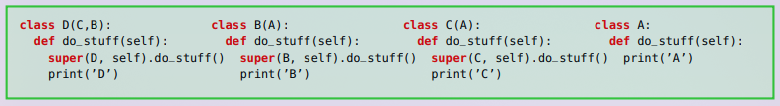
\includegraphics[scale=0.7]{3-OOP-1}
\end{center}

\textbf{Computing the method resolution order (MRO)}
\begin{itemize}
	\item if A is a superclass of B then B>A
	\item if C precedes D in the list of bases in a class statement then C>D
	\item if E>F in one scenario then E>F must hold in all scenarios
\end{itemize}

\begin{lstlisting}[language=Python]
[23:04]cazzola@hymir:~/esercizi-pa>python3
>>> from mro import A,B,C, D
>>> D.__mro__
(<class 'mro.D'>, <class 'mro.C'>, <class 'mro.B'>, <class 'mro.A'>, <class 'object'>)
>>> d = D()
>>> d.do_stuff()
A
B
C
D
\end{lstlisting}

\subsubsection{Special Methods}

\textbf{Special methods, as \_\_len\_\_(), \_\_str\_\_(), \_\_lt\_\_() and \_\_add\_\_(),
govern the behavior of some standard operations}

\begin{lstlisting}[language=Python]
class C(object):
	def __len__(self):
		return 0
def mylen():
	return 1
\end{lstlisting}

\begin{lstlisting}[language=Python]
[10:03]cazzola@hymir:~/pa>python3
>>> cobj = C()
>>> cobj.__len__ = mylen
>>> len(cobj)
0
\end{lstlisting}

\textbf{Special methods are “class methods”}
\begin{itemize}
	\item they cannot be changed through the instance
	\item this goes straight to the type by calling C.\_\_len\_\_()
\end{itemize}

\begin{lstlisting}[language=Python]
class C(object):
	def __len__(self): return self._mylen()
	def _mylen(self): return 0
def mylen():
	return 1
\end{lstlisting}

\begin{lstlisting}[language=Python]
[10:22]cazzola@hymir:~/pa>python3
>>> cobj = C()
>>> cobj._mylen = mylen
>>> len(cobj)
1
\end{lstlisting}

\textbf{To be more flexible}
- the special method must be forwarded to a method that can be overridden in the instance

\subsubsection{\_\_slots\_\_}

\textbf{Also built-in types, as list and tuple, can be subclassed}

\begin{lstlisting}[language=Python]
class MyList(list):
	"""A list that converts added items to ints"""
	def append(self, item):
		list.append(self, int(item))
	def __setitem__(self, key, item):
		list.__setitem__(self,key,int(item))
\end{lstlisting}

\begin{lstlisting}[language=Python]
[10:45]cazzola@hymir:~/esercizi-pa>python3
>>> l = MyList()
>>> l.append(1.3)
>>> l.append(444)
>>> l
[1, 444]
>>> len(l)
2
>>> l[1] = 3.14
>>> l
[1, 3]
\end{lstlisting}

\textbf{Unfortunately the subtype of list allow the adding of attributes}
- this is due to the presence of \_\_dict\_\_

\textbf{The presence of \_\_slots\_\_ in a class definition inhibits the introduction of \_\_dicts\_\_}
- this disallows any user-define attributes

\begin{lstlisting}[language=Python]
class MyList2(list):
	__slots__ = []
class MyList3(list):
	__slots__ = ['color']
class MyList4(list):
	"""A list that contains only ints"""
	def __init__(self, itr):
		list.__init__(self, [int(x) for x in itr])
	def append(self, item):
		list.append(self, int(item))
	def __setitem__(self, key, item):
		list.__setitem__(self,key,int(item))
\end{lstlisting}


\begin{lstlisting}[language=Python]
[11:13]cazzola@hymir:~/esercizi-pa>python3
>>> m2 = MyList2()
>>> m2.color = 'red'
Traceback (most recent call last):
File "<stdin>", line 1, in <module>
AttributeError:
'MyList2' object has no attribute 'color'
>>> m3 = MyList3()
>>> m3.color = 'red'
>>> m3.weight = 50
Traceback (most recent call last):
File "<stdin>", line 1, in <module>
AttributeError:
'MyList3' object has no attribute 'weight'
\end{lstlisting}